\section{Experiments}
\label{sec:Chapter_V}

This section answers four questions. How large is the gain from including yielding wait in the fitness (the closed loop)? How much further does reservation-table-aware dispatching reduce makespan, can it replace the closed loop, and do the two amplify each other when used together?
Over what range of instances do these gains hold, and \emph{can the present number of seeds determine} that range? Why do the other interfaces that we implemented fail to yield a net gain?

\subsection{Experimental setup}
\label{sec:instances}

\subsubsection{Controlled instance families}
FJSP\_PT benchmarks usually write travel times as a matrix indexed by location pairs; it records only the total duration between endpoints and supplies no corridor network.
Of the \PubNLayout{} layouts used by Homayouni and Fontes~\cite{homayouni2021production},
\PubNLayoutAsym{} matrices are entirely asymmetric (consistent with one-way tracks), and \PubNLayoutBad{} of them also violate the triangle inequality.
Asymmetry rules out undirected corridors of the kind used here (one $\tau_e$ per corridor, so the resulting $t^{*}$ must be symmetric);
violating the triangle inequality is stronger still: the all-pairs shortest paths of any graph satisfy the triangle inequality, so these \PubNLayoutBad{} matrices cannot be recovered even if directed graphs are allowed.
A network reverse-engineered from such a matrix would be a different instance, and the published reference values would no longer be comparable.
We therefore generate a set of controlled instances: the road network is given explicitly, and each feature of Section~\ref{sec:features} can be varied on its own.
A separate comparison on public instances---with the contention constraint removed, so that the problem reverts to the same mathematical problem as in the literature---is given in Section~\ref{sec:external}; it calibrates the strength of the upper-level search, not our framework.

All instances share the same core: $12$ jobs, $3$ operations per job for $36$ real operations, $8$ robotic arms,
heterogeneity $H=0.3$, and a transport-to-processing ratio $\bar{T}_t/\bar{T}_p$ scaled to $4.0$, so that vehicle contention is the main constraint.
$H$ is $0.3$ on all ten instances and does not vary with flexibility.
For each operation, the generator first draws independent perturbations of its $|\Omega_{ji}|$ processing times, standardizes them to zero mean and unit variance, and then multiplies them by $H$; the within-row coefficient of variation is therefore independent of $|\Omega_{ji}|$, and changing $F$ in Family~C does not change $H$.
Small deviations caused by rounding are measured after generation and recorded with each instance.
On this core, the instances vary along three factors (Table~\ref{tab:instances}).
Every instance is generated with a fixed random seed and is fully reproducible.

\emph{Family A: layout (contention structure).}
The first three instances use a spine layout: a main corridor (the spine) runs through the arm area, and each arm hangs off it on its own branch corridor at one of two hubs on the spine, half near the load/unload point $v_0$ and half at the far end of the spine; $v_0$ sits at one end of the spine and connects to it through one or two parallel exits.
This matches the spine layout common in high-volume plants---processing areas line both sides of a central corridor, in-plant moves travel along it, and congestion on that corridor is a known shop-floor problem~\cite{suh2022spine}.
Real shops usually place the store or load/unload point where the trips to all stations are roughly balanced, to shorten transport and spread corridor occupancy; we place $v_0$ at one end of the spine, so every transport must pass the same exit and the same stretch of the main corridor. This is a deliberately high-contention case, and it is exactly the case the closed-loop mechanism is meant to handle.
We also choose the spine layout because it concentrates contention on parallel lanes that can be added or removed: adding a lane changes capacity only, not distance. A tandem single-vehicle loop keeps vehicles from meeting each other~\cite{rahimikelarijani2020tandem}; it has almost no contention and does not suit the purpose of this study.

The spine layout covers only the high-contention range. Covering the low-contention range needs another topology, the \emph{grid}: with more intersections and more detours, an occupied corridor can be bypassed and contention falls, but the trip from the load/unload point to the farthest arm becomes longer.
The five instances therefore split into two topologies: \texttt{funnel}, \texttt{high}, and \texttt{mid} use the spine layout; \texttt{low} and \texttt{scatter} are grids.
Contention intensity runs from \ContentionAHi{} to \ContentionLo{}, but is not monotone in this construction order (\texttt{low} is above \texttt{mid}; per-instance values are in Table~\ref{tab:instances}).
The paper-wide maximum contention, \ContentionHi{}, is not in this family. It belongs to the instance that raises flexibility to $F=1.0$ (every operation may use every arm) on the same \texttt{funnel} layout, which is part of Family~C below.

The three spine instances differ only in their parallel lanes ($1\to2$ exits at the load/unload point, $1\to2$ lanes in the middle segment). Each lane is a two-hop path of equal total duration, so adding or removing one changes only how many vehicles can pass in parallel, not the distance; the node/corridor counts rise from $13/12$ to $15/16$.
\texttt{funnel} and \texttt{high} differ only by one parallel exit at the load/unload point, which halves the minimum cut; they form a single-factor contrast.
The two grid instances switch to a $4\times4$ grid ($16/24$), and to a scattered layout on the same grid that places the arms at the farthest points. The two have the same size and edge weights and differ only in arm placement; $v_0$ again sits at a corner.

The unimpeded trip from the load/unload point to the farthest arm is \LegDumbbell{} on all three spine instances and \LegGrid{} on both grid instances, nearly twice as long.
The two grid instances also have the highest makespans in the family, even though their contention intensity is the lowest.
This family is therefore a splice of ``capacity $+$ topology'', not an end-to-end single-factor scan: differences among the three spine instances can be attributed to capacity, while crossing over to the grid changes capacity and distance together.
When Section~\ref{sec:whichcongestion} orders the instances by contention intensity, two inversions appear: one stems from this topological splice, and the other lies inside the spine layout and needs a separate explanation.
Contention intensity is the quantity with which we directly describe congestion, and this family spans the widest range of it, so that section's judgement on where the closed loop applies rests mainly on this family.

\emph{Family B: vehicle-to-arm ratio $N_A/N_M$.}
On \texttt{funnel}, take $N_A\in\{4,8,12,16\}$, i.e.\ ratios of $0.5$, $1.0$, $1.5$, and $2.0$; $1.5$ is the base point shared by the three families (listed as \texttt{A funnel} under Family~A in the table).
This family tests whether dispatching has an upper limit in fleet size (Sections~\ref{sec:whichcongestion} and~\ref{sec:costlaw}).

\emph{Family C: flexibility $F$.}
On the same layout, take $F\in\{0.3,\,0.6,\,1.0\}$, i.e.\ the fraction of arms each operation may use; $0.6$ is again the base point.
$|\Omega_{ji}|$ is randomized and rounded so that its expectation equals $F\cdot N_M$; the measured base point is $0.61$ (Table~\ref{tab:instances} lists measured values; the other two levels match their targets).
Flexibility sets the scope of reassignment, and also how far corridor contention can be turned into an adjustment of the assignment.

The three families comprise $\NCases$ instances. The base point \texttt{A funnel} is at once the $1.5$ of Family~B and the $0.6$ of Family~C; it is generated and run only once, and occupies a single row in Tables~\ref{tab:instances} and~\ref{tab:bytag}.
Hence $5+3+2=\NCases$, while the Family~B and Family~C scans have four and three levels, respectively. Section~\ref{sec:whichcongestion} must count the base point when it reads these two families; leaving it out would make them look more monotone than they are.

Contention intensity is determined by the instance structure. It is measured on the initial random population ($20$ individuals) as the mean share of yielding wait in travel time; per-instance values are in Table~\ref{tab:instances}.
We do not use optimized solutions, because they reflect the solution rather than the instance: the search routes around congested corridors, contention tends to zero after convergence, and the differences among instances disappear.
Section~\ref{sec:whichcongestion} uses this quantity to order the instances.

\paragraph{Comparison with public instances.}
The $H$, $F$, and $\bar{T}_t/\bar{T}_p$ of our generated instances need an external reference.
The features of the \PubNInst{} public instances in Section~\ref{sec:external} are computed with the same feature function and the same convention, so the two can be compared directly.
Median flexibility is \PubFMed{}; our base point of $0.6$ is about one and a half times that, and the $F=0.3$ of Family~C falls inside the public range;
median heterogeneity is only \PubHMed{}, the largest of the \PubNInst{} instances is \PubHMax{}, and none reaches our $H=0.3$;
the public maximum of $\bar{T}_t/\bar{T}_p$ is only \PubTtTpHi{}, while we scale it to $4.0$.

The last two are both extrapolations, but with different meanings.
$\bar{T}_t/\bar{T}_p=4.0$ is deliberate: if transport is only a few percent of processing time, vehicle contention need not be modelled separately, and the common FJSP\_PT instances are of this kind.
$H=0.3$ lies above the literature range; if $H$ raised the closed-loop gain, part of the differences among configurations would come from this value.
Section~\ref{sec:whichcongestion} tests this with independent data spanning four levels of $H$, and the gain does not rise with $H$; the instances and baselines of that batch differ from the main batch, so it supports only this directional conclusion.

\begin{table}[t]
\caption{Controlled instances. All instances share $12$ jobs, $36$ real operations, $8$ robotic arms, $H=0.3$, and
$\bar{T}_t/\bar{T}_p\approx4.0$; the three families vary only the layout, the vehicle-to-arm ratio, and flexibility, respectively. Contention intensity is the share of yielding wait in total travel time on the initial
random population; it is determined by the instance structure and is not an input parameter.}
\label{tab:instances}
\small
%% 由 tab/gen_tables_ladder.py 生成:结构列直接由 tools/abc_matrix.py 的 build() 构造出
%% 算例后读出,下界调 algorithm/instance.py 的 simple_lower_bound,争用强度取自
%% baseline_ladder.csv 的 contention 列。任何一列都不是手打的。
%% 由 tab/gen_tables_ladder.py 生成,请勿手工编辑
%% 数据源:clbs/output/baseline_ladder.csv 等,见脚本首部
\begin{tabular}{@{}llrrrrrr@{}}
\toprule
Instance & Varied factor & Nodes & Corridors & $N_A$ & $F$ & Contention & Composite LB (time units) \\
\midrule
A funnel & layout & 13 & 12 & 12 & 0.61 & 31.9\% & 24.0 \\
A high & layout & 14 & 14 & 12 & 0.61 & 30.9\% & 17.0 \\
A low & layout & 16 & 24 & 12 & 0.61 & 11.8\% & 36.0 \\
A mid & layout & 15 & 16 & 12 & 0.61 & 10.8\% & 17.0 \\
A scatter & layout & 16 & 24 & 12 & 0.61 & 6.6\% & 36.0 \\
\midrule
B NA/NM 0.5 & $N_A/N_M$ & 13 & 12 & 4 & 0.61 & 15.8\% & 24.0 \\
B NA/NM 1.0 & $N_A/N_M$ & 13 & 12 & 8 & 0.61 & 30.2\% & 24.0 \\
B NA/NM 2.0 & $N_A/N_M$ & 13 & 12 & 16 & 0.61 & 32.4\% & 24.0 \\
\midrule
C F=0.3 & flexibility & 13 & 12 & 12 & 0.30 & 27.7\% & 24.0 \\
C F=1.0 & flexibility & 13 & 12 & 12 & 1.00 & 33.5\% & 24.0 \\
\bottomrule
\end{tabular}

\end{table}

\subsubsection{Comparison protocol}
\label{sec:protocol}

The comparison rests on the following rules.

\paragraph{Common executor: report the realized makespan.}
The makespan that the open loop schedules from unimpeded travel times is often infeasible on the real corridors.
Every configuration's schedule is therefore executed by the same conflict-free router and then checked by a validator independent of the decoder; what is compared is always the realized makespan after execution.
The gap between the open loop's self-reported and realized values (hereafter, the optimism margin) is especially large on the funnel layout.
If each configuration were compared on its own self-reported value, the open loop would gain an advantage from a makespan that cannot be realized.

\paragraph{Equal wall-clock budget, not equal generation count.}
A single evaluation does different work in each configuration: the open loop looks up the constant matrix $t^{*}$; the closed loop runs conflict-free routing for every candidate; the surcharge interface additionally needs a multi-label search.
The cost of a single evaluation can differ by about two orders of magnitude. Comparing at an equal generation count would give the more expensive configuration more compute, and an apparent mechanism gain might be only a larger budget.
We therefore align wall-clock time: all configurations on the same instance share the same budget, $90$ seconds in the main batch, with a cap of $2000$ generations and early stopping after $400$ consecutive generations without improvement.
The generation cap never fires. Every open-loop run is ended by early stopping after a little over four hundred generations, using on average about one fifth of the budget; both closed-loop configurations use the full $90$ seconds every time.
This setting favours the baseline: the open loop is not cut off by the budget but searches until it stops improving, and in its shorter wall-clock time it completes as many evaluations as closed-loop rule-based dispatching, or more (Section~\ref{sec:costlaw}).
Each remaining batch answers one specific question; their instances, seeds, and budgets are summarized in Table~\ref{tab:batches}.

\begin{table}[t]
\caption{Experiment batches. The main batch supports every statistical conclusion in Tables~\ref{tab:main} and~\ref{tab:bytag}; each other batch answers one specific question and is not set side by side with the main batch instance by instance.
``Speed-ups'' states whether the pruning and winner-path reuse of Section~\ref{sec:speedup} had been implemented. The surcharge mechanism and the yield-record-guided local search did not change before and after the speed-ups, and their cost is not affected by the pruning.}
\label{tab:batches}
\footnotesize
\begin{tabular}{@{}p{1.7cm}p{2.3cm}p{1.9cm}cp{1.6cm}c@{}}
\toprule
Batch & Purpose & Instances & Seeds & Wall-clock budget & Speed-ups \\
\midrule
Main & Four-level ladder (Tables~\ref{tab:main}, \ref{tab:bytag}) & Ten controlled instances & $\NSeeds$ & $90$\,s & yes \\
Cost diagnosis & Cost per evaluation (Figure~\ref{fig:protocol}) & Three controlled instances & $3$ & $90$\,s & yes \\
Convergence diagnosis & Convergence curves (Figure~\ref{fig:convergence}) & \texttt{funnel} & $3$ & $46.3$\,s & yes \\
Speed-up switch & Table~\ref{tab:prune} & Six controlled instances & $10$ & $90$\,s & off/on \\
Budget convention & Figure~\ref{fig:protocols} & Four instances & $10$ & Equal wall-clock and equal generations & no \\
Surcharge scan & Figure~\ref{fig:theta} & Two $8\times4\times4$ instances & $10$/$5$ & $48.9$/$60.7$\,s & no \\
Independent instances & Cross-check, $H$, ablations (Sections~\ref{sec:whichcongestion}, \ref{sec:pricing}) & $\MatrixCells$ instances & $10$ & $30.2$--$72.9$\,s & no \\
Public benchmarks & Table~\ref{tab:external} & $\PubNInst$ public instances & $\NSeeds$ & Early stopping & --- \\
\bottomrule
\end{tabular}
\end{table}

Aligning wall-clock time lets the configuration with the cheaper evaluation complete more evaluations.
Every configuration therefore reports both its cost per evaluation and the number of evaluations actually completed, and Section~\ref{sec:costlaw} analyses the trade-off between the two.

\paragraph{Seeds and paired tests.}
A single seed cannot support a conclusion: on the same instance and configuration, three seeds produced a range of $11$ makespan units, larger than any mechanism effect being measured.
Each instance is therefore run with $\NSeeds$ seeds, giving $\NCases\times\NSeeds=\NPairs$ pairs in total, and a two-sided Wilcoxon signed-rank test is performed with pairing by seed.
$\NSeeds$ seeds are enough to resolve an effect of a few percentage points when the $\NPairs$ pairs are pooled, but not inside a single instance.
Section~\ref{sec:whichcongestion} shows that this boundary falls exactly between the closed loop and dispatching; per-instance conclusions are confined to this power.

\paragraph{Multiple comparisons and effect sizes.}
The paper reports a little over twenty Wilcoxon tests. Without correction, the chance of ``at least one significant instance out of ten'' is about $40\%$ under the global null, not the nominal $5\%$.
Every family of tests is corrected within that family, and the family is stated where the result is reported.
There are two kinds of family: the five pooled contrasts of Table~\ref{tab:main} form one family; in Table~\ref{tab:bytag}, the $\NCases$ instances of each effect form one family.
We use the Holm correction to control the chance of at least one Type~I error within a family; Benjamini--Hochberg is computed as well, and any case where the two disagree is marked where it occurs.

There are two exceptions. First, when Section~\ref{sec:whichcongestion} reports the vehicle-to-arm ratio, it uses uncorrected $p$-values and marks each one: these values are already non-significant before correction, and correction would only make the conclusion more conservative.
Second, the independent data on \MatrixCells{} instances cited in Sections~\ref{sec:whichcongestion} and~\ref{sec:pricing} take their count of significant instances from that batch's own report, without correction under our rules; they serve only to confirm direction and magnitude, and every mention of that count should be read as an uncorrected count.
Apart from these two cases, every $p$-value in this paper is corrected.

Correction only answers whether the direction can be distinguished from zero. Each pooled contrast also reports a Hodges--Lehmann pseudomedian with a $95\%$ distribution-free confidence interval. These come from the same source as the Wilcoxon signed-rank test: the point estimate, the interval, and the $p$-value are all read from the same null distribution.
The mean pairwise relative gain, the main figure in our tables, is convenient for adding across tables, but it does not come from the rank test and carries no precision.
We give both. For example, the mean for dispatching inside the closed loop is \GainProbeLoop{} and the pseudomedian is \HLProbeLoop{}; the gap comes from pairs on the two vehicle-to-arm-ratio instances where makespan worsens (positive gain), and the pseudomedian is insensitive to such values.
Error bars in the figures are the standard error of the mean pairwise relative gain, shaded bands are the seed-to-seed range, and tables do not report $\pm$.

\paragraph{Correctness.}
For each solution, a validator independent of the decoder reconstructs the corridor occupancies from the timetable and compares the result with the composite lower bound.
Runs that fail the check or fall below the bound are reported separately and are not included in any instance mean.

\subsubsection{Implementation and environment}
\label{sec:impl}
The experiments run single-threaded on an Intel Xeon W-1270 @ $3.40$\,GHz. The implementation is pure Python ($\ge 3.9.6$) using only the standard library, with no third-party dependencies and no solver.
The hyperparameters of the outer genetic algorithm and the local search take their defaults, are not tuned, and are identical across configurations: population $60$, crossover probability $0.8$, mutation probability $0.2$, elite $5$, binary tournament; the local search acts each generation on the top $10\%$ of individuals, examines at most $L=5$ critical operations per round, and runs at most three rounds.
Because the hyperparameters are conventional and identical across configurations, the measured gains come from the mechanisms rather than from operator tuning.
Absolute runtimes cannot be compared with those of a compiled implementation. A faster implementation would let every configuration complete more evaluations within the same budget, but would not change the ratio of cost per evaluation between configurations; this ratio is measured between configurations that share the same implementation.

\subsection{Four-level baseline ladder}
\label{sec:arms}

The comparison must answer two questions separately: how much the makespan differs when the structure is aligned with the pipeline structures common in the literature, and how much it differs when only one component is changed.
The former requires structural correspondence; the latter requires changing one thing at a time.
Ablations alone cannot be mapped onto the common pipeline structures, while a literature comparison alone would credit the gain of conflict-free routing itself to our mechanisms.
We therefore use a four-level ladder in which each level corresponds to a clearly identifiable structure.

\begin{description}[leftmargin=0pt,topsep=3pt,itemsep=3pt]
\item[B0: open-loop planning + realized execution.]
The upper level searches by unimpeded shortest-path times (the search ignores conflicts); after the search, the plan is executed by the same conflict-free router.
This represents the open-loop structure: the scheduling layer produces a plan that ignores transport contention, and a downstream conflict-free router executes it. FJSP\_PT methods that schedule on a constant matrix~\cite{meng2025cp,qin2026knowledge,fu2025integrated} fall into this class when executed on a real road network, as does the framework of Li et al.~\cite{li2026framework}. Dispatching is idle-first, the same as Eq.~\eqref{eq:rule} used by rule-based dispatching in our framework.
\item[B0+: open-loop planning + reservation-table-aware dispatching.]
The schedule is likewise fixed by unimpeded travel times; only vehicle selection is changed to a trial query on the reservation table.
This represents the two-stage structure: the first stage schedules on a \emph{constant travel-time matrix}, and only the second stage optimizes vehicle assignment and handles conflicts on the fixed schedule, with no feedback (e.g.\ Sun et al.~\cite{sun2023integrated}).
Here, reservation-table-aware dispatching serves as a greedy approximation of that second stage.
\item[B1: closed-loop planning + rule-based dispatching.]
Fitness during the search is taken from conflict-free routing, while dispatching still estimates times from unimpeded shortest paths via Eq.~\eqref{eq:rule}. It differs from B2 only in the vehicle-selection rule.
\item[B2: closed-loop planning + reservation-table-aware dispatching.]
Our method.
\end{description}

The four levels are in fact a $2\times2$ design along two factors, not a linear sequence. The first factor is whether the search includes conflict-induced delay (open-loop / closed-loop); the second is whether a vehicle is selected by unimpeded time or by a trial query on the reservation table (rule / trial query).
If two configurations differ in both factors at once, their difference cannot be decomposed.
For example, $\text{B0+}\to\text{B1}$ crosses both factors and \textbf{cannot} be used to measure the closed loop.
The interpretable contrasts fix one factor and change only the other, i.e.\ the four pairs that share a row or a column of Table~\ref{tab:arms}.

\begin{table}[t]
\caption{The $2\times2$ structure of the four-level ladder. Rows: whether the search includes conflict-induced delay; columns: whether a vehicle is selected by unimpeded time or by a trial query on the reservation table.
Comparisons within a row or a column differ in one factor; a diagonal comparison changes both and cannot be decomposed.}
\label{tab:arms}
\footnotesize
\begin{tabular}{@{}lcc@{}}
\toprule
 & Rule-based dispatching & Reservation-table-aware dispatching \\
\midrule
Open loop (schedule first, then route; search ignores conflicts) & B0 & B0+ \\
Closed-loop planning (fitness from conflict-free routing) & B1 & \textbf{B2} (ours) \\
\bottomrule
\end{tabular}
\end{table}

How B0 is executed decides how strong the baseline is. The plan found by the open-loop search already contains a set of vehicle assignments, and it can be reproduced at execution time in two ways:
\emph{replay the plan} executes with the vehicles the original plan specifies; \emph{on-site reassignment} re-selects vehicles by the rule at execution time.
The former is measured to be stronger ($63.00$ versus $78.00$ on the funnel instance) and matches the practice of Li et al.~\cite{li2026framework}, whose task-allocation layer fixes the robots on the Gantt chart first and, at execution, only shifts the time axis without reassignment.
The main report uses the stronger replay-the-plan convention; on-site reassignment is listed alongside.

\subsection{Aggregate comparison on the ladder}
\label{sec:main}

Table~\ref{tab:main} gives the makespans of the four-level ladder over $\NCases$ instances $\times$ $\NSeeds$ seeds, i.e.\
$\NPairs$ pairs in total, with the same wall-clock budget on each instance (Section~\ref{sec:protocol}); every run passed the independent check.
The next three paragraphs read the effect along each of the two factors, and then the pooled $\text{B0}\to\text{B2}$.
The $p$-values in the table are Holm-corrected over these five contrasts, and the correction changes no decision.
The text reports pseudomedians and confidence intervals as \emph{reductions}; Table~\ref{tab:main} shows the same intervals as negative values.

\begin{table}[t]
\caption{Makespans of the four-level ladder under an equal wall-clock budget, and the four pairs that change only one thing along the two factors.
A negative value means a lower makespan, i.e.\ better. $n=\NPairs$ comparisons paired by $(\text{instance},\text{seed})$,
two-sided Wilcoxon signed-rank tests; $p$-values are Holm-corrected over the five contrasts of this table
($^{*}p<0.05$, $^{**}p<0.01$, $^{***}p<0.001$). The HL column is the Hodges--Lehmann
pseudomedian of pairwise relative gains with its $95\%$ distribution-free confidence interval (see Section~\ref{sec:protocol}).
A bold header marks our configuration; numbers are not bold because B2 is not best on every instance (per-instance results in Table~\ref{tab:bytag}).}
\label{tab:main}
\small
%% 由 tab/gen_tables_ladder.py 从 clbs/output/baseline_ladder.csv 生成。该脚本同时打印
%% 导言区的整块宏定义,故表与正文的数字必然同源:重跑实验后只需重跑脚本、贴一次宏。
%% 已核实脚本独立复现出导言区当前的全部数值(增益、p 值、胜负计数、争用区间)。
%% 2026-08-20:p 列改为 Holm 校正后的值,并加印 HL 伪中位数与 95% CI。校正对这五个对比是
%% 惰性的:最大的一个 p 恰为最大者、乘数为 1,其余小到乘 5 仍远低于阈值,故数字不变而口径变严。
%% 由 tab/gen_tables_ladder.py 生成,请勿手工编辑
%% 数据源:clbs/output/baseline_ladder.csv 等,见脚本首部
\begin{tabular}{@{}lrrrrr@{}}
\toprule
& & \multicolumn{4}{c}{$C_{\max}$ (time units)} \\
\cmidrule(lr){3-6}
Instance & Contention & B0 & B0$^{+}$ & B1 & \textbf{B2} \\
\midrule
A funnel & 31.9\% & 58.10 & 53.50 & 44.70 & 42.40 \\
A high & 30.9\% & 56.00 & 51.40 & 39.90 & 37.70 \\
A low & 11.8\% & 64.50 & 64.60 & 57.80 & 57.10 \\
A mid & 10.8\% & 46.40 & 42.70 & 39.40 & 37.40 \\
A scatter & 6.6\% & 62.30 & 62.30 & 57.20 & 57.10 \\
\midrule
B NA/NM 0.5 & 15.8\% & 71.00 & 70.50 & 69.00 & 65.10 \\
B NA/NM 1.0 & 30.2\% & 56.70 & 56.50 & 47.50 & 49.80 \\
B NA/NM 2.0 & 32.4\% & 70.60 & 64.20 & 42.20 & 44.20 \\
\midrule
C F=0.3 & 27.7\% & 74.30 & 69.50 & 51.60 & 47.30 \\
C F=1.0 & 33.5\% & 52.10 & 47.50 & 39.30 & 36.30 \\
\midrule
\emph{Pooled mean} & --- & 61.20 & 58.27 & 48.86 & 47.44 \\
\bottomrule
\end{tabular}

\vspace{0.6em}

\begin{tabular}{@{}lrlrr@{}}
\toprule
Single-factor paired contrast & $\Delta C_{\max}$ & HL pseudomedian and $95\%$ CI (\%) & W/L/T & $p_{\mathrm{Holm}}$ \\
\midrule
Closed-loop value (rule-based) & $-18.86\%^{***}$ & $-18.28$ $[-21.95,-14.68]$ & 96/2/2 & $<10^{-4}$ \\
Closed-loop value (reservation-table-aware) & $-17.75\%^{***}$ & $-18.00$ $[-20.55,-15.22]$ & 93/5/2 & $<10^{-4}$ \\
Dispatching value (open-loop) & $-4.59\%^{***}$ & $-4.45$ $[-6.13,-2.88]$ & 68/19/13 & $<10^{-4}$ \\
Dispatching value (closed-loop) & $-2.45\%^{**}$ & $-3.03$ $[-5.19,-0.94]$ & 60/34/6 & $0.0054$ \\
\midrule
\textbf{End-to-end: literature $\rightarrow$ this paper} & $-21.35\%^{***}$ & $-21.20$ $[-24.46,-17.99]$ & 94/5/1 & $<10^{-4}$ \\
\bottomrule
\end{tabular}

\end{table}

\paragraph{Closed-loop evaluation.}
Fixing the vehicle-selection rule and changing only whether the search includes conflict-induced delay, the closed loop is significantly better under both dispatching rules: under rule-based dispatching,
$\text{B0}\to\text{B1}$ is $-\GainLoopRule$ ($p\PLoopRule$); under reservation-table-aware dispatching,
$\text{B0+}\to\text{B2}$ is $-\GainLoopProbe$ ($p\PLoopProbe$).
For the former, the Hodges--Lehmann pseudomedian is \HLLoopRule{} with $95\%$ confidence interval \CILoopRule{}. The whole interval lies far from zero and even its lower end is a two-digit reduction, so this level does not depend on whether the point estimate is a mean or a pseudomedian.
The gap cannot be explained by the number of evaluations, because that difference runs the other way: an open-loop evaluation only looks up a constant matrix, so within the same budget the open loop completes several times as many evaluations as the closed loop (the cost per evaluation of each configuration is shown in Figure~\ref{fig:protocol}).
The open loop evaluates more and is still worse, because it optimizes a surrogate objective that excludes yielding; the true transport cost appears only after the plan is fixed.
Figure~\ref{fig:convergence} shows this gap on a single instance.

The closed loop is significant under both dispatching rules, so this conclusion does not depend on our vehicle-selection rule.

\begin{figure}[t]
\centering
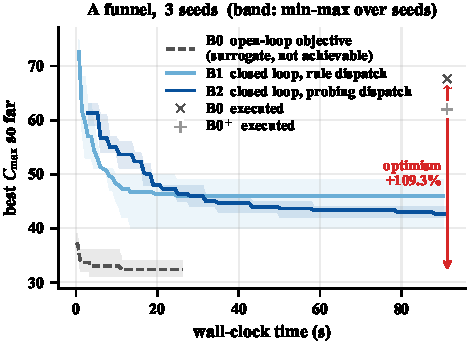
\includegraphics[width=\columnwidth]{fig/fig_convergence_closedloop.pdf}
\Description{Best-so-far makespan against wall-clock time for the ladder
configurations, with the open-loop curve marked as a surrogate objective and its
realizable value shown as a separate point. Each curve carries a shaded band
giving the min-to-max range across the three seeds.}
\caption{Convergence curves on a single \texttt{funnel} instance (taken from a diagnostic batch of three instances). The horizontal axis is wall-clock time; each curve is the time-wise mean over three seeds,
and the shaded band is the seed-to-seed \emph{range} (the sample is too small to estimate quartiles).
The solid lines (B1, B2) are always realized makespans; the dashed line is the surrogate objective of the open-loop search, i.e.\ the quantity it actually optimizes;
crosses and pluses mark the makespan of the same plan after execution by conflict-free routing.
The gap between the end of the dashed line and the cross is the optimism margin on this instance: the open loop has not failed to converge; it has converged to a surrogate objective that cannot be realized.
The figure is illustrative and supports no statistical conclusion (see Table~\ref{tab:batches} for the batch).}
\label{fig:convergence}
%% 由 fig/fig_convergence_CN.py 生成(输出名 fig_convergence_closedloop_CN),
%% 数据源 clbs/output/ladder_convergence.csv 与 ladder_cost.csv,由 tools/ladder_diag.py 落盘。
%% 该图是说明性的:它画形状与落差,不承载统计主张,故只取三算例三种子,正文统计一律以
%% baseline_ladder.csv 为准。此口径已写在 ladder_diag.py 的首部注释里。
\end{figure}

\paragraph{Reservation-table-aware dispatching.}
Fix the open or closed loop and change only the vehicle-selection rule. \emph{Inside the closed loop},
$\text{B1}\to\text{B2}$ is $-\GainProbeLoop$ ($p\PProbeLoop$), with pseudomedian \HLProbeLoop{} and
$95\%$ confidence interval \CIProbeLoop{}.
The two levels share the same scheduling search and the same budget; they differ only in whether vehicle selection uses a trial query on the reservation table.
This is a pooled result. The interval does not cross zero, but its lower end is less than one percentage point from zero; after family-wise correction no instance is significant (\CellsSigProbe{} before correction), and two of the ten instances have a positive sign, i.e.\ B2 is slower than B1 at vehicle-to-arm ratios $1.0$ and $2.0$ (Table~\ref{tab:bytag}).
Thus $-\GainProbeLoop$ is an average effect over this instance family and cannot be applied instance by instance;
Section~\ref{sec:whichcongestion} discusses this resolution limit.

\emph{Under the open loop}, the same rule gives $-\GainProbeOpen$ ($p\PProbeOpen$), likewise significant.
It measures the step from the open-loop structure to the two-stage structure;
its magnitude (\GainProbeOpen{}) is far smaller than that of the closed loop (\GainLoopRule{}).
Reservation-table-aware dispatching is significant under both the open and the closed loop, but its effect is much smaller and cannot by itself explain the $\text{B0}\to\text{B2}$ reduction.

\paragraph{End to end, and how the two effects combine.}
\label{sec:complement}
$\text{B0}\to\text{B2}$ is $-\GainEndToEnd$ when pooled
($p\PEndToEnd$; of the $\NPairs$ pairs, $\WinEndToEnd$ wins, $\LoseEndToEnd$ losses, and $1$ tie).
That is, moving from open-loop planning with rule-based dispatching to closed-loop planning with reservation-table-aware dispatching lowers makespan by about one fifth. The three effects have different reference points, so they cannot simply be added.
If the closed loop and dispatching were independent, the end-to-end gain would equal the compound of the closed loop under rule-based dispatching ($\GainLoopRule$) and dispatching under the open loop ($\GainProbeOpen$), i.e.\ $\GainIndepProduct$. The measured $\GainEndToEnd$ is slightly below this, which shows that each mechanism contributes on its own and \emph{the two do not amplify each other}: B2 is best end to end because the two gains add up.

\paragraph{Relation to ``schedule first, then resolve conflicts''.}
Dispatching still yields a significant $\GainProbeOpen$ under the open loop, so the shortfall of this approach lies not in second-stage dispatching but in the first stage ignoring yielding. Placed in a two-stage structure, the same dispatching rule gains only as much as open-loop dispatching, far less than the closed loop's $\GainLoopRule$; to obtain the closed-loop reduction, yielding wait must enter the fitness during the search. These gaps were measured on our instance families.

\subsection{Three-factor scans and per-instance resolution}
\label{sec:whichcongestion}

The aggregate comparison of Section~\ref{sec:main} rests on $\NCases$ instances. This section takes them apart by layout, vehicle-to-arm ratio, and flexibility.
The trend of the closed loop can be read by family; dispatching cannot be distinguished from zero on any single instance. This section reports that difference. Each of the three families corresponds to an expectation that can be stated in advance.

\emph{Layout (Family A)} tests whether the gain grows with contention intensity: both paths target the delay caused by vehicles yielding to one another, and when contention is weak this delay is small, so their effect is limited.

\emph{Vehicle-to-arm ratio (Family B)} tests whether there is an upper bound on fleet size beyond which overhead offsets the gain. Trial-query cost grows approximately linearly with the fleet, and the pruning of Section~\ref{sec:speedup} has its lowest cut rate on the instance with the largest fleet.

\emph{Flexibility (Family C)} tests whether the gain depends on room for reassignment.

\paragraph{Per-instance resolution.}
The significance marks of Table~\ref{tab:bytag} decide which instances may be read by sign.
If each of the $\NCases$ instances is tested once, the probability of ``at least one significant'' under the global null is far above $5\%$.
Per-instance tests therefore receive a Holm correction by family, the family being the $\NCases$ instances of one effect (the closed loop and dispatching each form a family; they answer different questions and are not merged into one family of twenty tests).
The marks in Table~\ref{tab:bytag} and Figure~\ref{fig:prediction3} are all based on the corrected $p$.

After correction the closed loop remains significant on \CellsSigLoopAdj{} instances (\CellsSigLoop{} before correction; the largest corrected value is $p\PLoopCellMax$, so the verdict does not depend on the correction). The only exception is the instance with the fewest vehicles ($\text{B0}\to\text{B1}$ is \GainLoopStarve{}, not significant). The trend of the closed loop can therefore be read by family.
Dispatching inside the closed loop is significant on \CellsSigProbe{} instances before correction (the two ends of the flexibility family, $p\PProbeFlexLoRaw$ and $p\PProbeFlexHiRaw$), and \emph{on \CellsSigProbeAdj{} instances after correction}: Holm gives $p\PProbeFlexLoHolm$ and $p\PProbeFlexHiHolm$, and Benjamini--Hochberg gives $p\PProbeFlexLoBH$ and $p\PProbeFlexHiBH$, likewise not significant.
No instance reaches significance on its own. The effect size (a few percentage points) is of the same order as the smallest effect that $\NSeeds$ seeds on one instance can resolve. Only the $\NPairs$ pooled pairs separate it from noise, and only just: the pseudomedian is \HLProbeLoop{}, and the $95\%$ interval \CIProbeLoop{} does not cross zero, with its lower end less than one percentage point from zero.
Below, per-instance results for dispatching are reported as directions only; the sign is judged only on the pooled data.

\begin{table}[t]
\caption{Per-instance results of the four-level ladder and the two effects, closed loop and dispatching, blocked by the three families (each instance has $n=\NSeeds$ comparisons paired by seed).
Significance marks follow the \textbf{Holm-corrected} $p$ (two-sided Wilcoxon signed-rank test), the family being the
$\NCases$ instances of one effect: $^{*}p<0.05$, $^{**}p<0.01$; $^{\dagger}$ means significant before correction but not after, and the sign of that instance is not taken as a conclusion.
A negative value means a lower makespan. The two gain columns use the same estimator as Table~\ref{tab:main} (the mean of pairwise relative gains over seeds) and cannot be obtained by dividing the two means in the same row.
\texttt{A funnel} is at once $N_A/N_M=1.5$ of Family~B and $F=0.6$ of Family~C; it is run only once and occupies only one row.}
\label{tab:bytag}
\small
%% 由 tab/gen_tables_ladder.py 生成,按 A/B/C 三族分块。
%% 逐格增益列已于 2026-08-16 从"两档均值之比"改为"逐对相对增益的均值",与 tab_main 及
%% 导言区宏同源;同时加印显著性标记,因为下文按格读符号。
%% 标记已于 2026-08-20 改按 Holm 校正后的 p 值,并为"校正前显著、校正后不显著"的格加印
%% 剑号。改动只影响标记,不影响任何增益数字;受影响的格是柔性族两格(试探列)。
%% 由 tab/gen_tables_ladder.py 生成,请勿手工编辑
%% 数据源:clbs/output/baseline_ladder.csv 等,见脚本首部
\begin{tabular}{@{}lrrrrrrr@{}}
\toprule
& & \multicolumn{4}{c}{$C_{\max}$ (time units)} & \multicolumn{2}{c}{Pairwise relative gain} \\
\cmidrule(lr){3-6}\cmidrule(lr){7-8}
Instance & Contention & B0 & B0$^{+}$ & B1 & \textbf{B2} & B0$\rightarrow$B1 & B1$\rightarrow$B2 \\
\midrule
A funnel & 31.9\% & 58.10 & 53.50 & 44.70 & 42.40 & $-21.3\%^{*}$ & $-4.6\%$ \\
A high & 30.9\% & 56.00 & 51.40 & 39.90 & 37.70 & $-26.6\%^{*}$ & $-4.8\%$ \\
A low & 11.8\% & 64.50 & 64.60 & 57.80 & 57.10 & $-10.3\%^{*}$ & $-1.1\%$ \\
A mid & 10.8\% & 46.40 & 42.70 & 39.40 & 37.40 & $-14.4\%^{*}$ & $-4.8\%$ \\
A scatter & 6.6\% & 62.30 & 62.30 & 57.20 & 57.10 & $-8.1\%^{*}$ & $+0.1\%$ \\
\midrule
B NA/NM 0.5 & 15.8\% & 71.00 & 70.50 & 69.00 & 65.10 & $-2.0\%$ & $-4.7\%$ \\
B NA/NM 1.0 & 30.2\% & 56.70 & 56.50 & 47.50 & 49.80 & $-15.6\%^{*}$ & $+5.0\%$ \\
B NA/NM 2.0 & 32.4\% & 70.60 & 64.20 & 42.20 & 44.20 & $-37.7\%^{*}$ & $+5.7\%$ \\
\midrule
C F=0.3 & 27.7\% & 74.30 & 69.50 & 51.60 & 47.30 & $-29.7\%^{*}$ & $-8.2\%^{\dagger}$ \\
C F=1.0 & 33.5\% & 52.10 & 47.50 & 39.30 & 36.30 & $-22.9\%^{*}$ & $-7.2\%^{\dagger}$ \\
\bottomrule
\end{tabular}

\end{table}

\begin{figure}[t]
\centering
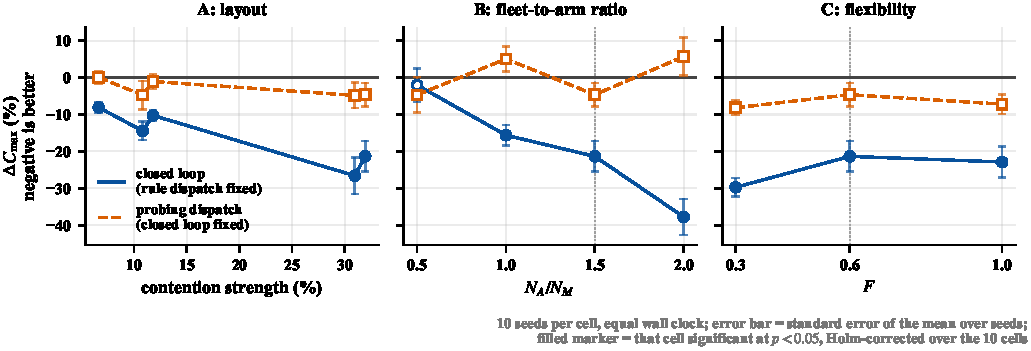
\includegraphics[width=\columnwidth]{fig/fig_prediction3.pdf}
\Description{Three panels of line plots: closed-loop gain and reservation-aware
dispatch gain across layout (vs contention), fleet-to-arm ratio, and flexibility. After
Holm correction over the ten cells the closed-loop curve is filled, hence
significant, at nine of ten cells, while the dispatch curve is hollow at every
cell, and its sign alternates across the four fleet-ratio levels. Error bars
give the standard error of the mean over the ten seeds of each cell; the
dispatch bars cross zero at every cell and the closed-loop bars do not.}
\caption{The closed loop and dispatching across the three families. Left: layout family, horizontal axis contention intensity; middle: vehicle-to-arm ratio, $N_A/N_M$; right: flexibility.
Families~B and~C include the shared base point ($1.5$ and $0.6$, at the hollow vertical lines), which is also listed as \texttt{A funnel} in Family~A.
Filled markers remain significant after Holm correction ($p<0.05$, the family being the $\NCases$ instances of one effect); hollow markers are not significant.
Error bars are the standard error of the mean of pairwise relative gains over the $\NSeeds$ seeds of each instance.
The closed loop is significant on \CellsSigLoopAdj{} instances and rises roughly with contention; after correction dispatching is significant on \emph{no instance}, its error bars cross zero on every instance, and its sign alternates across the four levels of the vehicle-to-arm ratio.
The point of the figure is whether the two curves can be distinguished from zero, not the shape of the dispatching curve.}
\label{fig:prediction3}
%% 由 fig/fig_prediction3_CN.py 从 clbs/output/baseline_ladder.csv 生成。横轴:A 族取争用强度
%% (布局族没有自然的数值水平,而布局操纵改变的正是争用),B/C 族取算例名末尾的因子水平——
%% 那个数字由 tools/abc_matrix.py 生成算例时写入,故按构造即为水平本身;基点 A funnel 的
%% 名字里没有水平,其 (1.5, 0.6) 由脚本按 abc_matrix.BASE 显式补入,见脚本内注释。
%% 标记的实心/空心由逐格 Wilcoxon 的 p 值决定。上一版按增益是否为正标注 "harmful",
%% 那等于把不显著的符号当成结论,现已改为按显著性区分标记。
%% 2026-08-20:填充判据改为 Holm 校正后的 p 值,族取该效应的全部十格(而不是当前面板的
%% 三到五格,否则共用基点会因所在面板不同而得到两种填充)。改动后试探那条曲线全为空心。
\end{figure}

Table~\ref{tab:bytag} and Figure~\ref{fig:prediction3} give the per-instance results. The three families are read differently.

\emph{Layout family.}
The closed loop rises roughly with contention intensity and is significant on all five instances: on the least congested \texttt{scatter} (contention \ContentionLo{}), $\text{B0}\to\text{B1}$ is \GainLoopScatter{}; on \texttt{mid}/\texttt{low} it is \GainLoopMid{}/\GainLoopLow{}; on \texttt{funnel}/\texttt{high} it is \GainLoopFunnel{}/\GainLoopHigh{}.
We say ``roughly'' because there are two inversions of different kinds.
\texttt{low} has higher contention than \texttt{mid} but a smaller gain. The two lie on opposite sides of the topological boundary of Section~\ref{sec:instances} (grid versus spine, farthest trip \LegGrid{} versus \LegDumbbell{}), so this is not a pure contention inversion.
\texttt{funnel} has higher contention than \texttt{high} but a smaller gain. Both are spine instances that differ only by one parallel exit at the load/unload point, the planned single-factor contrast, so \emph{this inversion is a counter-example}.
What can be established is the magnitude (\GainLoopFunnel{} on the most congested instance versus \GainLoopScatter{} on the least congested, about two and a half times), not a monotone relation between contention and gain.
Contention intensity summarizes congestion as a single number and does not separate the part that reassignment can bypass; see Limitation (1) in Section~\ref{sec:limitations}.
Dispatching is not significant on any instance of this family, so only its direction is reported: four of the five instances are negative, the same direction as the closed loop.

\emph{Vehicle-to-arm-ratio family.}
This family does not establish an upper bound of applicability for dispatching. Dispatching inside the closed loop at the four levels is, in order, $-\GainProbeStarve$ ($N_A/N_M=0.5$), \GainProbeFleetOne{} ($1.0$), \GainProbeFleetBase{} ($1.5$, the base point \texttt{A funnel}), and \GainProbeFleetTwo{} ($2.0$). The sign alternates, and none of the four instances is significant ($p\PProbeFleetHalfRaw$, $p\PProbeFleetOneRaw$, $p\PProbeFleetBaseRaw$, $p\PProbeFleetTwoRaw$; these are values \emph{before} correction, already non-significant).
Taking only the three levels $0.5$, $1.0$, and $2.0$, the curve shows the monotone rise predicted by the cost law; once the base point in the middle is included, this trend no longer holds.
The upper bound predicted in Section~\ref{sec:costlaw} therefore remains untested: testing it would require enough seeds to resolve effects of a few percentage points, which exceeds the budget of this paper.
The closed loop at $1.0$ and $2.0$ is \GainLoopFleetOne{} and \GainLoopFleetTwo{}, both significant: fleet size mainly affects the closed-loop gain, not dispatching.

\emph{Flexibility family.}
After Holm correction, the dispatching effect is not significant in this family either.
At $F=0.3$, $0.6$, and $1.0$, dispatching is \GainProbeFlexLo{}, \GainProbeFleetBase{}, and \GainProbeFlexHi{}. The three have the same sign, and the two ends are the two largest magnitudes among all $\NCases$ instances (the base point falls back to a level comparable with the rest). The raw values at the two ends, $p\PProbeFlexLoRaw$ and $p\PProbeFlexHiRaw$, rise after correction to $p\PProbeFlexLoHolm$ and $p\PProbeFlexHiHolm$, which are no longer significant.
This family provides only directional evidence, of the same sign as the pooled result and of the largest magnitude.
The same sign at all three levels, without the sign alternation of the vehicle-to-arm-ratio family, is compatible with ``dispatching acts mainly through vehicle selection and timing, and does not depend strongly on the number of eligible arms'': if dispatching relied on room for reassignment, $F=0.3$ should fail first, yet it is the instance with the largest magnitude.
The closed loop is \GainLoopFlexLo{} and \GainLoopFlexHi{}, still significant per instance after correction.

\paragraph{An independent batch of self-generated instances.}
The results above come from one instance family and one baseline. As a cross-check we use another batch of self-generated instances with contention (public benchmarks are treated in Section~\ref{sec:external}, where contention has been removed): $\MatrixCells$ instances $\times$ $10$ seeds, $\MatrixRuns$ runs in all.
Both the instance core and the baseline differ: the baseline is two-stage surrogate transport, and the batch crosses four contention levels with four heterogeneity levels.
The \emph{integration gain} (two-stage $\to$ closed-loop) is \GainIntegMatrix{}, significant on \SigIntegMatrix{} of the $\MatrixCells$ instances and ranging from \GainIntegMatrixLo{} to \GainIntegMatrixHi{}, consistent in direction and magnitude with the closed loop in this section.
Counts of significant instances in this batch are uncorrected (see Section~\ref{sec:protocol}).

\paragraph{Heterogeneity does not raise the closed-loop gain.}
The four $H$ levels of that batch answer the question left open in Section~\ref{sec:instances}. Grouping the $\MatrixCells$ instances into four levels by $H$ (four instances per level, one at each contention level), the integration gain is \GainIntegHZero{} at $H=0$, \GainIntegHLow{} at $H=0.15$ (measured \MatrixHMeasLow{}), \GainIntegHMid{} at $H=0.3$, and \GainIntegHHigh{} at $H=0.5$; the rank correlation between gain and $H$ is a weakly negative \RhoIntegH{}.

The measured $H=\MatrixHMeasLow$ lies near the public-instance median \PubHMed{}, and its gain \GainIntegHLow{} differs from the \GainIntegHMid{} at $H=0.3$ by less than half a percentage point: setting $H$ above the literature range did not raise the closed-loop gain.
The expectation that the gain rises with $H$ does not hold: the trend is not monotone, and the rank correlation is negative. Each level has only $4$ instances, and the within-level spread (\GainIntegMatrixLo{} to \GainIntegMatrixHi{}) is far larger than the gaps between levels. The data therefore support only ``the gain does not rise with $H$'' and are not sufficient to assert that $H=0.5$ is lower.
This is compatible with the analysis of Section~\ref{sec:features}: as $H$ grows, processing-time differences among eligible arms gradually outweigh differences in corridor accessibility, so assignment is decided more and more by processing speed and less and less by traffic conditions.
$H=0$ removes the trade-off, not the opportunity: all arms in $\Omega_{ji}$ have the same processing time, so reassignment need not trade processing time for travel time and becomes a pure congestion decision at zero cost. This level has the highest gain of the four (\GainIntegHZero{}), consistent with the definition.
Thus $H$ turns arm selection into a trade-off (without heterogeneity, the reversal of Section~\ref{sec:Chapter_I} would not occur), but it does not amplify the closed-loop gain. The closed-loop gain comes from whether the search accounts for yielding; contention strength is set by layout and fleet, not by $H$.

For reservation-table-aware dispatching, that batch gives \GainProbePre{} ($0$ instances significant), the opposite direction from the main batch. The batch ran before the two speed-ups; see Section~\ref{sec:costlaw} for the reason.

